\documentclass[manuscript,screen,review]{acmart}


\IfFileExists{upquote.sty}{\usepackage{upquote}}{}
\IfFileExists{microtype.sty}{% use microtype if available
  \usepackage[]{microtype}
  \UseMicrotypeSet[protrusion]{basicmath} % disable protrusion for tt fonts
}{}
\makeatletter
\@ifundefined{KOMAClassName}{% if non-KOMA class
  \IfFileExists{parskip.sty}{%
    \usepackage{parskip}
  }{% else
    \setlength{\parindent}{0pt}
    \setlength{\parskip}{6pt plus 2pt minus 1pt}}
}{% if KOMA class
  \KOMAoptions{parskip=half}}
\makeatother

%%
%% This is file `sample-manuscript.tex',
%% generated with the docstrip utility.
%%
%% The original source files were:
%%
%% samples.dtx  (with options: `manuscript')
%% 
%% IMPORTANT NOTICE:
%% 
%% For the copyright see the source file.
%% 
%% Any modified versions of this file must be renamed
%% with new filenames distinct from sample-manuscript.tex.
%% 
%% For distribution of the original source see the terms
%% for copying and modification in the file samples.dtx.
%% 
%% This generated file may be distributed as long as the
%% original source files, as listed above, are part of the
%% same distribution. (The sources need not necessarily be
%% in the same archive or directory.)
%%
%%
%% Commands for TeXCount
%TC:macro \cite [option:text,text]
%TC:macro \citep [option:text,text]
%TC:macro \citet [option:text,text]
%TC:envir table 0 1
%TC:envir table* 0 1
%TC:envir tabular [ignore] word
%TC:envir displaymath 0 word
%TC:envir math 0 word
%TC:envir comment 0 0
%%
%%
%% The first command in your LaTeX source must be the \documentclass command.


% Options for packages loaded elsewhere
\PassOptionsToPackage{unicode}{hyperref}
\PassOptionsToPackage{hyphens}{url}
\PassOptionsToPackage{dvipsnames,svgnames,x11names}{xcolor}

\IfFileExists{bookmark.sty}{\usepackage{bookmark}}{\usepackage{hyperref}}

%% PANDOC PREAMBLE BEGINS


\providecommand{\tightlist}{%
  \setlength{\itemsep}{0pt}\setlength{\parskip}{0pt}}\usepackage{longtable,booktabs,array}
\usepackage{calc} % for calculating minipage widths
% Correct order of tables after \paragraph or \subparagraph
\usepackage{etoolbox}
\makeatletter
\patchcmd\longtable{\par}{\if@noskipsec\mbox{}\fi\par}{}{}
\makeatother
% Allow footnotes in longtable head/foot
\IfFileExists{footnotehyper.sty}{\usepackage{footnotehyper}}{\usepackage{footnote}}
\makesavenoteenv{longtable}
\usepackage{graphicx}
\makeatletter
\def\maxwidth{\ifdim\Gin@nat@width>\linewidth\linewidth\else\Gin@nat@width\fi}
\def\maxheight{\ifdim\Gin@nat@height>\textheight\textheight\else\Gin@nat@height\fi}
\makeatother
% Scale images if necessary, so that they will not overflow the page
% margins by default, and it is still possible to overwrite the defaults
% using explicit options in \includegraphics[width, height, ...]{}
\setkeys{Gin}{width=\maxwidth,height=\maxheight,keepaspectratio}
% Set default figure placement to htbp
\makeatletter
\def\fps@figure{htbp}
\makeatother

\usepackage{booktabs}
\usepackage{longtable}
\usepackage{array}
\usepackage{multirow}
\usepackage{wrapfig}
\usepackage{float}
\usepackage{colortbl}
\usepackage{pdflscape}
\usepackage{tabu}
\usepackage{threeparttable}
\usepackage{threeparttablex}
\usepackage[normalem]{ulem}
\usepackage{makecell}
\usepackage{xcolor}
\definecolor{mypink}{RGB}{219, 48, 122}
\makeatletter
\@ifpackageloaded{caption}{}{\usepackage{caption}}
\AtBeginDocument{%
\ifdefined\contentsname
  \renewcommand*\contentsname{Table of contents}
\else
  \newcommand\contentsname{Table of contents}
\fi
\ifdefined\listfigurename
  \renewcommand*\listfigurename{List of Figures}
\else
  \newcommand\listfigurename{List of Figures}
\fi
\ifdefined\listtablename
  \renewcommand*\listtablename{List of Tables}
\else
  \newcommand\listtablename{List of Tables}
\fi
\ifdefined\figurename
  \renewcommand*\figurename{Figure}
\else
  \newcommand\figurename{Figure}
\fi
\ifdefined\tablename
  \renewcommand*\tablename{Table}
\else
  \newcommand\tablename{Table}
\fi
}
\@ifpackageloaded{float}{}{\usepackage{float}}
\floatstyle{ruled}
\@ifundefined{c@chapter}{\newfloat{codelisting}{h}{lop}}{\newfloat{codelisting}{h}{lop}[chapter]}
\floatname{codelisting}{Listing}
\newcommand*\listoflistings{\listof{codelisting}{List of Listings}}
\makeatother
\makeatletter
\makeatother
\makeatletter
\@ifpackageloaded{caption}{}{\usepackage{caption}}
\@ifpackageloaded{subcaption}{}{\usepackage{subcaption}}
\makeatother
%% PANDOC PREAMBLE ENDS

\setlength{\parindent}{10pt}
\setlength{\parskip}{0pt}

\hypersetup{
  pdftitle={Changing Beliefs About Correlations in Atypical Scatterplots},
  pdfauthor={Gabriel Strain; Andrew J. Stewart; Paul Warren; Charlotte Rutherford; Caroline Jay},
  colorlinks=true,
  linkcolor={blue},
  filecolor={Maroon},
  citecolor={Blue},
  urlcolor={red},
  pdfcreator={LaTeX via pandoc, via quarto}}

%% \BibTeX command to typeset BibTeX logo in the docs
\AtBeginDocument{%
  \providecommand\BibTeX{{%
    Bib\TeX}}}

%% Rights management information.  This information is sent to you
%% when you complete the rights form.  These commands have SAMPLE
%% values in them; it is your responsibility as an author to replace
%% the commands and values with those provided to you when you
%% complete the rights form.
\setcopyright{acmcopyright}
\copyrightyear{2018}
\acmYear{2018}
\acmDOI{XXXXXXX.XXXXXXX}

%% These commands are for a PROCEEDINGS abstract or paper.
\acmConference[Conference acronym 'XX]{Make sure to enter the correct
conference title from your rights confirmation emai}{June 03--05,
2018}{Woodstock, NY}
\acmPrice{15.00}
\acmISBN{978-1-4503-XXXX-X/18/06}

%% Submission ID.
%% Use this when submitting an article to a sponsored event. You'll
%% receive a unique submission ID from the organizers
%% of the event, and this ID should be used as the parameter to this command.
%%\acmSubmissionID{123-A56-BU3}

%%
%% For managing citations, it is recommended to use bibliography
%% files in BibTeX format.
%%
%% You can then either use BibTeX with the ACM-Reference-Format style,
%% or BibLaTeX with the acmnumeric or acmauthoryear sytles, that include
%% support for advanced citation of software artefact from the
%% biblatex-software package, also separately available on CTAN.
%%
%% Look at the sample-*-biblatex.tex files for templates showcasing
%% the biblatex styles.
%%

%%
%% The majority of ACM publications use numbered citations and
%% references.  The command \citestyle{authoryear} switches to the
%% "author year" style.
%%
%% If you are preparing content for an event
%% sponsored by ACM SIGGRAPH, you must use the "author year" style of
%% citations and references.
%% Uncommenting
%% the next command will enable that style.
%%\citestyle{acmauthoryear}


%% end of the preamble, start of the body of the document source.
\begin{document}


%%
%% The "title" command has an optional parameter,
%% allowing the author to define a "short title" to be used in page headers.
\title{Changing Beliefs About Correlations in Atypical Scatterplots}

%%
%% The "author" command and its associated commands are used to define
%% the authors and their affiliations.
%% Of note is the shared affiliation of the first two authors, and the
%% "authornote" and "authornotemark" commands
%% used to denote shared contribution to the research.


  \author{Gabriel Strain}
  \orcid{0000-0002-4769-9221}
            \affiliation{%
                  \institution{Department of Computer Science, Faculty
of Science and Engineering, University of Manchester}
                          \streetaddress{Oxford Road}
                          \city{Manchester}
                                  \country{United Kingdom}
                          \postcode{M13 9PL}
              }
        \author{Andrew J. Stewart}
  
            \affiliation{%
                  \institution{Department of Computer Science, Faculty
of Science and Engineering, University of Manchester}
                          \streetaddress{Oxford Road}
                          \city{Manchester}
                                  \country{United Kingdom}
                          \postcode{M13 9PL}
              }
        \author{Paul Warren}
  
            \affiliation{%
                  \institution{Division of Psychology, Communication and
Human Neuroscience, School of Health Sciences, Faculty of Biology,
Medicine, and Health, University of Manchester}
                          \streetaddress{Oxford Road}
                          \city{Manchester}
                                  \country{United Kingdom}
                          \postcode{M13 9PL}
              }
        \author{Charlotte Rutherford}
  
            \affiliation{%
                  \institution{Division of Psychology Communication and
Human Neuroscience, School of Health Sciences, Faculty of Biology,
Medicine, and Health, University of Manchester}
                          \streetaddress{Oxford Road}
                          \city{Manchester}
                                  \country{United Kingdom}
                          \postcode{M13 9PL}
              }
        \author{Caroline Jay}
  
            \affiliation{%
                  \institution{Department of Computer Science, Faculty
of Science and Engineering, University of Manchester}
                          \streetaddress{Oxford Road}
                          \city{Manchester}
                                  \country{United Kingdom}
                          \postcode{M13 9PL}
              }
      
\renewcommand{\shortauthors}{Strain et al.}

%% By default, the full list of authors will be used in the page
%% headers. Often, this list is too long, and will overlap
%% other information printed in the page headers. This command allows
%% the author to define a more concise list
%% of authors' names for this purpose.
%\renewcommand{\shortauthors}{Trovato et al.}
%%  
%% The abstract is a short summary of the work to be presented in the
%% article.
\begin{abstract}
abstract goes here    
\end{abstract}

%%
%% The code below is generated by the tool at http://dl.acm.org/ccs.cfm.
%% Please copy and paste the code instead of the example below.
%%
\begin{CCSXML}
<ccs2012>
 <concept>
  <concept_id>10010520.10010553.10010562</concept_id>
  <concept_desc>Computer systems organization~Embedded systems</concept_desc>
  <concept_significance>500</concept_significance>
 </concept>
 <concept>
  <concept_id>10010520.10010575.10010755</concept_id>
  <concept_desc>Computer systems organization~Redundancy</concept_desc>
  <concept_significance>300</concept_significance>
 </concept>
 <concept>
  <concept_id>10010520.10010553.10010554</concept_id>
  <concept_desc>Computer systems organization~Robotics</concept_desc>
  <concept_significance>100</concept_significance>
 </concept>
 <concept>
  <concept_id>10003033.10003083.10003095</concept_id>
  <concept_desc>Networks~Network reliability</concept_desc>
  <concept_significance>100</concept_significance>
 </concept>
</ccs2012>
\end{CCSXML}

\ccsdesc[500]{Computer systems organization~Embedded systems}
\ccsdesc[300]{Computer systems organization~Redundancy}
\ccsdesc{Computer systems organization~Robotics}
\ccsdesc[100]{Networks~Network reliability}

%%
%% Keywords. The author(s) should pick words that accurately describe
%% the work being presented. Separate the keywords with commas.
\keywords{belief change, correlation
perception, scatterplot, crowdsourced}


%%
%% This command processes the author and affiliation and title
%% information and builds the first part of the formatted document.
\maketitle

\setlength{\parskip}{-0.1pt}

\section{Introduction}\label{sec-intro-main}

Utilized for communication in a wide variety of contexts, scatterplots
are simple representations of (usually) bivariate data. They were
estimated in 1983 to account for between 70 and 80 percent of data
visualizations in scientific publications \citep{tufte_1986}, and while
there is no doubt that the range of data visualizations employed in and
beyond science is now far broader, scatterplots remain an important tool
for the data visualization designer. The appeal of researching
scatterplots lies in evidence that people generally interpret them in
similar ways \citep{kay_2015}, that they are interpreted rapidly
\citep{rensink_2014}, and that they are ubiquitous in both academic
\citep{tufte_1986} and non-academic contexts.

While most commonly used to communicate the linear correlation, or level
of relatedness, between a pair of variables, scatterplots can also be
designed to facilitate the detection of outliers, to convey differences
between clusters, or to display non-linear correlations. The suitability
of scatterplots to such a range of tasks, and the opportunity for
designers to design with a multitude of tasks in mind, plays a large
part in their popularity. Building on previous work, we elect to focus
on the use of scatterplots for the communication of linear, bivariate,
positive correlation. There is evidence that, while correlation
perception in scatterplots experiences low levels of interindividual
variance (especially when compared to other visualizations that
communicate the same idea {[}\citet{harrison_2014}; kay\_2015{]}), our
accuracy in interpretation is poor. Studies asking participants to
numerically estimate correlation
\citep{strahan_1978, bobko_1979, cleveland_1982, lane_1985, lauer_1989, collyer_1990, meyer_1992}
or estimate it via a bisection task \citep{rensink_2017} find consistent
levels of underestimation, particularly when 0.2 \textless{} \emph{r}
\textless{} 0.6. If scatterplots were used solely for communication
between those trained in statistics and data visualization, this would
not be especially problematic, however this is not the case; lay people
being expected to be able to use and interpret data visualizations on an
almost daily basis. It is thus the duty of those who design such
visualizations to design with the naive, inexperienced viewer in mind.
Doing so requires us to understand \emph{how} visualizations work, and
to gain an appreciation for the hidden processes that allow pictorial
representations to convey much more than words and numbers ever could.

Recent work has sought to address the correlation underestimation bias
in positively correlated scatterplots through the use of novel point
encodings. In 2023 and 2024, Strain et al.
\citep{strain_2023, strain_2023b, strain_2024} began exploiting the idea
that viewers use the width of a probability distribution conveyed by the
arrangement of scatterplot points as a proxy for their judgements of
correlation to successfully (albeit partially) correct for the
underestimation bias. As of the time of writing, this work has only
provided evidence about perceptual effects using a simple direct
estimation paradigm, and while successful, has not investigated whether
these techniques can influence cognition in the context of real-world
data visualizations and the relatedness between variables. As doing this
is crucial for providing designers with the tools to design
visualizations that are adapted for the facilitation of more accurate
correlation perception, we therefore present a two experiment study
investigating the propensity for recently established scatterplot
visualization techniques to bias participant's beliefs about levels of
relatedness between variables.

\begin{itemize}
\tightlist
\item
  and has seen success by using point size and opacity manipulations
\item
  as of writing, this work has only provided evidence about perceptual
  effects using a simple estimation paradigm
\item
  and has not investigated whether these effects can extend to cognition
  about relatedness between real variables
\item
  this is important wrt the potential for using the manipulations to
  improve visualisations
\item
  we present a 2 experiment study in which we first use novel research
  methods and crowdsourcing to select a statement about relatedness that
  is agreed upon (phrasing), then we test the propensity for previously
  described visual manipulations to alter beliefs about relatedness,
  taking into account various additional participant qualities.
\end{itemize}

\section{Related Work}\label{sec-rel-work-main}

In this section we briefly discuss related work on correlation
perception and estimation, the history and current state of the use of
point size and opacity adjustments in scatterplots, including how these
visual features have been used with regards to correction for the
underestimation bias, and perception and cognition in data
visualization. We then review the literature around belief change as it
pertains to data visualization, before ending with our hypotheses for
the present study.

\subsection{Correlation Perception}\label{correlation-perception}

Correlation describes the level of relatedness between a number of
variables. There are a number of different types of correlation, however
in this work, we use the term to refer to Pearson's \emph{r}, which
takes a positive or negative value between 0 and 1 depending on the
direction of the relationship being described. Mechanistically, evidence
is inconclusive regarding what drives correlation perception in
scatterplots, however some experimental results point towards the shape
of the underlying probability distribution as a likely candidate.
Scatterplots with smaller point clouds produce increased judgements of
correlation \citep{cleveland_1982}, suggesting that it is the area of
the point cloud that may influence perception. Work exploring the
relationship between subjective and objective \emph{r} values in
scatterplots found that this relationship could be described by a power
function that included the mean of the geometrical distances between
scatterplot points and a regression line. Other work includes some
representation of the shape of a scatterplot's point cloud in equations
describing magnitude estimation and correlation discrimination
\citep{meyer_1997, rensink_2017}, and work on visual features as proxies
for correlation found that a similar quantity again is predictive of
performance. While we cannot say that this \emph{is} the process of
correlation perception in scatterplots, we can conclude that the shape
of the point cloud is a good proxy for what is really occurring during
judgements of correlation.

\subsection{Scatterplots: Size, Opacity, and Recent
Developments}\label{scatterplots-size-opacity-and-recent-developments}

The idea that it is the shape of the point cloud, and the probability
distribution it represents that is being used to inform judgements of
correlation has received support from recent work exploiting visual
features with the intention of making correlation estimation more
accurate. Strain et al. \citep{strain_2023, strain_2023b, strain_2024},
used functions that changed the sizes and opacities of points in
scatterplots as a function of their distance from the regression line,
and achieved success in biasing correlation estimates in positive and
negative directions. When point opacities \citep{strain_2023} or point
sizes \citep{strain_2023b} were reduced with residual distance,
participants were significantly more accurate on a correlation
estimation task; employing both of these manipulations simultaneously
\citep{strain_2024} resulted in an overshoot of correction, biasing
participants further. \textbf{?@fig-previous-manipulations} contains a
summary of previously tested scatterplot manipulations and their effects
on performance on a correlation estimation task

\subsection{Perception \& Cognition in Data
Visualization}\label{perception-cognition-in-data-visualization}

\subsection{Persuasion \& Belief Change in Data
Visualization}\label{persuasion-belief-change-in-data-visualization}

\begin{itemize}
\tightlist
\item
  Correlation Perception Testing Drivers
\item
  Scatterplots Opacity Adjustments in Scatterplots Point Size
  Adjustments in Scatterplots
\item
  Perception \& Cognition in Data Visualization Differences between them
  Why study the extension from one to the other? Beliefs changing as a
  result of viewing visualisations the persuasive power of data viz why
  this is important over just presenting numbers maybe something
  specifically about scatterplots lead onto the primary motivation of
  this study hypotheses- statement
\end{itemize}

\section{General Methods}\label{sec-general-methods}

In this section we discuss our general research methods, including our
implementations of open research practices, our approach to and
justification for crowdsourcing, and our use of the ChatGPT4 LLM in
preparing parts of our stimuli.

\subsection{Open Research}\label{sec-open-research}

Both our pre and main studies were conducted according to the principles
of open and reproducible research \citep{ayris_2018}. We pre-registered
hypotheses and analysis plans with the Open Science Framework (OSF) for
the pre-study\footnote{The GitHub repository associated with this paper
  contains an R script that performs this analysis.} and the main
experiment\footnote{removed for anon}, and there were no deviations from
them. All data and analysis code are included in a GitHub
repository\footnote{removed for anon}. This repository contains
instructions for building a Docker container \citep{merkel_2014} that
reproduces the computational environment the paper was written in. This
allows for full replication of stimuli, figures, analysis, and the paper
itself. Ethical approval was granted by the (removed for anon).

\subsection{Crowdsourcing}\label{crowdsourcing}

While much prior work into correlation perception in scatterplots has
taken place in person, there is precedence for work that explores
cognition to take place online using crowdsourced participants
\citep{xiong_2022}. Crowdsourcing not only affords us recruitment of
samples from across our lay population of interest, it is considerably
quicker and less expensive than in-person testing. We therefore choose
to crowdsource all participants. Previous work has reported issues of
data quality and skewed demographics
\citep{chmielewski_2020, charalambides_2021, peer_2021}, so we follow
published guidelines \citep{peer_2021} to give us the best chance of
collecting high quality data. We use the Prolific.co platform
\citep{prolific} with strict pre-screening criteria; participants were
required to have completed at least 100 studies using Prolific, and were
required to have a Prolific score of 100, representing a 99\% approval
rate.

\subsection{Use of Large Language
Models}\label{use-of-large-language-models}

\begin{itemize}
\tightlist
\item
  issues regarding stimulus generation normally
\item
  advantages conferred by using ChatGPT
\item
  reproducibility issues?
\end{itemize}

\section{Pre-Study: Investigating Beliefs About Relatedness
Statements}\label{sec-pre-study}

\subsection{Introduction}\label{sec-pre-study-intro}

\subsubsection{Testing Beliefs}\label{sec-testing-beliefs}

\subsubsection{Preparation of Stimuli}\label{sec-stim-prep-pre}

Due to previous evidence suggesting effects of prior belief strength and
topic emotionality on the propensity for belief change, we first aim to
build a picture of people's thoughts and feelings along these dimensions
in our population of interest. With the intention of testing the
potential for changes in beliefs about correlations displayed in
scatterplots depicting weak and strong correlations, and those whose
topics were both strong and neutral in emotional valence, we began by
using ChatGPT4 \citep{chatgpt} to generate 100 correlation statements
using the following prompt:

\begin{flushleft}

    ``Generate 100 statements that describe the correlation between two variables, such as :

     "X is associated with a higher level of Y" or

     "As X increases, Y increases".

    Try to match all the statements on emotionality.``
    
\end{flushleft}

The full list of these statements can be found in the supplementary
materials. Note that we cite our use of ChatGPT according to the AI Code
of Conduct developed by Iliada Eleftheriou and Ajmal Mubarik and the
University of Manchester \citep{iliada_2023}. Two authors rated each
statement on topic emotionality and strength of correlation using Likert
scales from 1 to 7. Topic emotionality had a midpoint at 4, whereas
strength of correlation varied between 1 (Not Related At All) and 7
(Strongly Related). We calculated a quadratic weighted Cohen's Kappa
between the two raters using the \textbf{irr} package (version 0.84.1
\citep{irr}), in order to penalise larger magnitude disagreements more
harshly. We found agreement above chance for both topic emotionality
(\(\kappa\) = 0.49, \emph{p} \textless{} .001) and strength of
correlation (\(\kappa\) = 0.51, \emph{p} \textless{} .001), indicating
moderate levels of agreement in both cases
\citep{cohen_1968, fleiss_1969}.

\begin{table}

\caption{\label{tbl-pre-test-hi}Pre-test statements that were rated as
being strongly correlated.}

\centering{

\begin{tabular}[t]{rl}
\toprule
Item Number & Statement - Strong Correlation Depicted\\
\midrule
1 & Increased exposure to sunlight is correlated with higher vitamin D levels.\\
2 & As caffeine consumption increases, so does the average heart rate.\\
3 & Greater frequency of exercise is linked to a lower risk of depression.\\
4 & Greater use of helmets is associated with a lower incidence of head injuries in cyclists.\\
5 & As the quality of healthcare improves, life expectancy tends to increase.\\
\addlinespace
6 & As access to clean water improves, the incidence of waterborne diseases decreases.\\
7 & Higher levels of empathy are linked to stronger interpersonal relationships.\\
8 & As soil quality degrades, agricultural productivity tends to decrease.\\
9 & Higher levels of civic engagement are linked to a stronger sense of community.\\
10 & Higher sugar consumption is associated with an increased risk of dental cavities.\\
\addlinespace
11 & Higher attendance at preventive health screenings is linked to earlier detection of diseases.\\
12 & Increased use of energy-efficient appliances is associated with lower electricity bills.\\
13 & As pedestrian-friendly infrastructure improves, urban walkability tends to increase.\\
14 & Greater regularity in sleep patterns is associated with improved mental health.\\
\bottomrule
\end{tabular}

}

\end{table}%

\begin{table}

\caption{\label{tbl-pre-test-low}Pre-test statements that were rated as
being weakly correlated.}

\centering{

\begin{tabular}[t]{rl}
\toprule
Item Number & Statement - Weak Correlation Depicted\\
\midrule
15 & Greater water consumption is linked to improved kidney function.\\
16 & As the amount of sleep decreases, the risk of obesity increases.\\
17 & Greater intake of omega-3 fatty acids is associated with lower inflammation levels.\\
18 & Greater exposure to music education is linked to enhanced cognitive development in children.\\
19 & Higher exposure to air conditioning is associated with increased respiratory issues.\\
\addlinespace
20 & Higher frequency of family meals is linked to better eating habits in children.\\
21 & As participation in community arts programs increases, local cultural engagement tends to rise.\\
22 & Higher consumption of spicy foods is associated with a lower risk of certain types of cancer.\\
23 & Greater adherence to a Mediterranean diet is linked to a lower risk of neurodegenerative diseases.\\
24 & Higher consumption of nuts and seeds is associated with reduced risk of cardiovascular diseases.\\
\addlinespace
25 & As cultural preservation efforts increase, community identity and cohesion tend to strengthen.\\
\bottomrule
\end{tabular}

}

\end{table}%

Following this, we selected strongly and weakly correlated statements
with the highest level of absolute agreement, resulting in the 14
strongly correlated statements that can be seen in
Table~\ref{tbl-pre-test-hi} and the 11 weakly correlated statements that
can be seen in Table~\ref{tbl-pre-test-low}. We then tested these 25
statements with a representative UK sample in order to ascertain
consensus on both topic emotionality and strength of correlation. Doing
so allows us to effectively exclude these factors when we analyse the
effects of our atypical scatterplot designs on the propensity for belief
change in our main experiment.

\subsection{Method}\label{sec-method-pre}

\subsubsection{Participants}\label{sec-participants-pre}

100 participants were recruited using the Prolific.co platform
\citep{prolific}. English fluency and residency was required for
participation, as our main experiment relied on familiarity with data
visualizations from a popular British news source. In addition to 25
experimental items, we included six attention check items, which asked
participants to provide specific answers. No participants failed more
than 2 out of 6 attention check items, and therefore data from all 100
were included in the full analysis (52.0\% male and 48.0\% female.
Participants' mean age was 41.1 (\emph{SD} = 12.3). The average time
taken to complete the survey was 7.6 minutes (\emph{SD} = 2.9 minutes).

\subsubsection{Design}\label{sec-design-pre}

Each participant saw all survey items (Table~\ref{tbl-pre-test-hi} and
Table~\ref{tbl-pre-test-low}), along with the six attention check items,
in a fully randomised order. All experimental code, materials, and
instructions are hosted on GitLab\footnote{https://gitlab.pavlovia.org/Strain/beliefs\_scatterplots\_pretest}.

\subsubsection{Procedure}\label{sec-procedure-pre}

The experiment was built using Psychopy \citep{pierce_2019} and hosted
on Pavlovia.org. Participants were permitted to complete the experiment
using a phone, tablet, desktop, or laptop computer. Participants were
first shown the participant information sheet and were asked to provide
consent through key presses in response to consent statements. They were
asked to provide their age in a free text box, followed by their gender
identity. Participants were told that they would be asked to read
statements about the relatedness between a pair of variables, after
which they would have to indicate their beliefs about topic emotionality
and the strength of correlation suggested using a pair of sliders. To
familiarize themselves with the sliders, they were asked to complete a
practice round in response to the statement ``As participation in online
experiments increases, society becomes happier.''

\subsection{Results}\label{sec-results-pre}

All analyses were conducted using R (version 4.4.1). We use the
\textbf{irr} package to calculate Fleiss' Kappa to measure interrater
agreement on topic emotionality and strength of correlation for the 25
experimental items. This analysis revealed that participants agreed
above chance for both topic emotionality (\(\kappa\) = 0.07, \emph{p}
\textless{} .001) and strength of correlation (\(\kappa\) = 0.06,
\emph{p} \textless{} .001).

\subsection{Selecting Statements for the Main
Experiment}\label{selecting-statements-for-the-main-experiment}

To control for any potential effects of topic emotionality in the main
experiment, we first select statements that represent neutral emotional
valence. Statements with average topic emotionality ratings between 3
and 5 are statements 2, 10, 22, 16, and 23. To ascertain which
statements represent the greatest consensus, we add standard deviations
in ratings for topic emotionality and strength of correlation. Due to
concerns about experimental power, and in line with evidence that
propensity for belief change is highest when prior beliefs are not
strongly held \citep{xiong_2022}, we elected at this point to test only
the statement corresponding to weak beliefs about the strength of
correlation between the variables in question. We therefore test
statement number 22, ``Higher consumption of spicy foods is associated
with a lower risk of certain types of cancer.'', however we modify the
wording so that both variables (food consumption and cancer risk) are
positively correlated, as previous work indicates that the manipulations
we use in the atypical scatterplot condition are able to change
estimates of correlation in positively correlated scatterplots; no work
regarding the effects of these manipulations in negatively correlated
scatterplots has been completed.

\subsection{Discussion}\label{sec-discussion-pre}

Fleiss' Kappa values for interrater agreement on both topic emotionality
and strength of correlation scales are low (\(\kappa\) = 0.07 and
\(\kappa\) = 0.06 respectively), however do exceed that which would be
expected by chance. We suggest this may be due to Fleiss' Kappa not
being designed with ordinal (Likert scales in this case) data in mind.
In light of this we do not make decisions regarding which statement to
use based on the values of Fleiss' Kappa observed, but rather on the
standard deviations of ratings across all raters. Regardless, we do not
consider this to be a particular weakness, as we also test topic
emotionality and strength of correlation with participants in the main
study and include these ratings as part of our analysis.

\section{Main Study: Potential for Belief Change Using Atypical
Scatterplots}\label{sec-main-study}

We test the statement that exhibited the lowest average level of belief
about correlation, and the 2nd highest level of consensus. Modified for
directionality, this statement is therefore: ``Higher consumption of
plain (non-spicy) foods is associated with a lower risk of certain types
of cancer.''

\subsection{Introduction}\label{introduction}

\begin{itemize}
\tightlist
\item
  hypotheses
\item
\end{itemize}

\subsubsection{Defensive Confidence}\label{defensive-confidence}

In line with evidence that those who are more confident in their ability
to defend their own positions are more susceptible to having those
positions changed \citep{albarracin_2004}, we test participants'
defensive confidence using a 12-item scale. This scale is replicated
from previous work in the supplemental material, and has additionally
been utilized more recently \citep{markant_2023} to explore the
potential for attitude change specifically with regards to correlations
in scatterplots. Participants provide answers to the 12 scale items
using a 5 point Likert scale ranging from 1 (\emph{not at all
characteristic of me}) to 5 (\emph{extremely characteristic of me}).
Analysis including participants' defensive confidence scores is included
in \textbf{?@sec-additional-analyses}.

\subsection{Stimuli}\label{stimuli}

Recent work has shown that estimates of correlation can be altered when
point opacities and sizes are systematically varied in scatterplots
\citep{strain_2023, strain_2023b, strain_2024}. These manipulations have
been used in an attempt to correct for a long-standing underestimation
bias observed in correlation perception as it pertains to scatterplots.
As we now aim to test the propensity of these manipulations to affect
participants' beliefs about levels of relatedness, we choose the set of
manipulations that has previously produced the most dramatic effect on
correlation estimates; namely, the combination of typical orientation
size and opacity manipulations provided by Strain et al
\citep{strain_2024}. Here, the size and opacity of a certain scatterplot
point is lowered as a function of that point's residual error using
equation 1:

\begin{equation}
  point_{size/opacity} = 1 - b^{residual}
\end{equation}

In order to facilitate comparison to this work, we use the same protocol
to produce scatterplots for our atypical condition. This includes
creating scatterplots with 128 points, using \emph{b} = 0.25, employing
a scaling factor and constant for point size, and using an opacity floor
to ensure point visibility, as this has been an issue in previous work.
As there is evidence that people are less likely to update strongly held
beliefs following viewing scatterplot visualizations \citep[ look for
more]{markant_2023}, we selected a correlative statement that was judged
as representing weakly correlated variables. Thus, in order to induce
belief change, participants only viewed scatterplots representing
\textbf{strongly} correlated variables (0.6 \textgreater{} \emph{r}
\textgreater{} 0.99). We used \textbf{ggplot} in R to create plots that
echoed the style of a British news broadcaster and fictitiously claimed
the data to be provided by the British National Health service. Examples
of typical and atypical data-identical scatterplots can be seen in
\textbf{?@fig-main-examples}.

\begin{figure}

\centering{

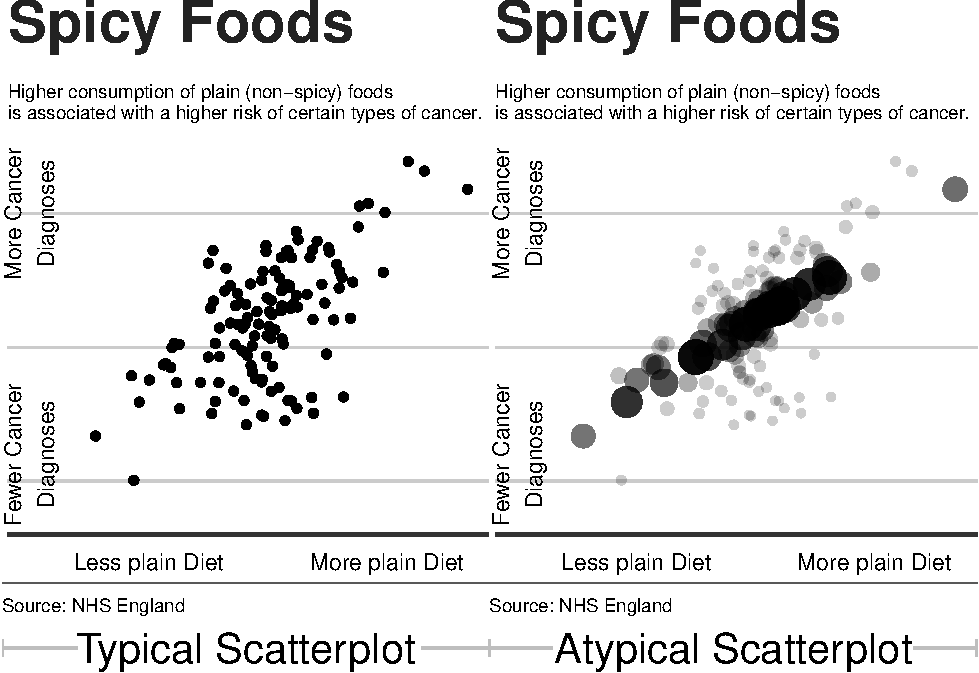
\includegraphics[width=1\textwidth,height=\textheight]{beliefs_attitudes_atypical_scatterplots_files/figure-pdf/fig-example-plots-1.pdf}

}

\caption{\label{fig-example-plots}Examples of the experimental stimuli
used with an \textit{r} value of 0.6.}

\end{figure}%

\subsection{Method}\label{method}

\subsubsection{Participants}\label{participants}

Participants were recruited using Prolific.co \citep{prolific}. English
fluency and UK residency was required for participation, as well as
normal or corrected-to-normal vision, and having not participated in any
of our previous studies regarding correlation perception in scatterplots
\citep{strain}, as these represented earlier testing of the alternative
designs we employ in the atypical scatterplot condition. Data were
collected from 77 participants for each condition. 2 participants failed
more than 2 out of 4 attention check questions for each condition,
meaning their data were excluded per pre-registration stipulations. Data
from the remaining 150 participants were included in the full analysis
(48.7\% male, 48.7\% female, and 2.7\% non-binary). Participants' mean
age was 39.3 (\emph{SD} = 11.5). Participants' mean graph literacy score
was 21.3 (\emph{SD} = 4.3) out of 30, their mean defensive confidence
score was 43.0 (\emph{SD} = 6.8) out of 60, and their mean rating of
topic emotionality was 2.9 (\emph{SD} = 1.3) on a 7 point Likert scale.
On average, participants took 14.2 minutes to complete the experiment
(\emph{SD} = 6.41).

\subsubsection{Design}\label{design}

We employed a between-participants design. Each participants was
randomly assigned to either group A, in which case they viewed typical
scatterplots, or group B, in which they viewed atypical scatterplots
designed deliberately to elicit higher levels of belief change.
Participant saw all experimental items for their group, along with 4
attention check items, in a fully randomised order. All experimental
code, materials, and instructions are hosted on GitLab as two separate
experiments \footnote{The GitHub repository associated with this paper
  contains an R script that performs this analysis.} \footnote{removed
  for anon}

\subsubsection{Procedure}\label{procedure}

We use PsychoPy \citep{pierce_2019} to build our experiment and
Pavlovia.org to host it. Participants were permitted to complete the
experiment on a desktop or laptop computer. We elected to prevent
participants from using a phone or tablet to complete the experiment in
line with evidence that differences in on-screen sizes of data
visualizations can alter perceptions {[}cleveland\_1982{]}. Participants
were first shown the participant information sheet and asked to provide
consent through key presses in response to consent statements. They
were, again, asked to provide their age and gender identity.
Participants then completed the 12-item Defensive Confidence scale
described by Albarracín and Mitchell \citep{albarracin_2004} and the
5-item Subjective Graph Literacy scale \citep{garcia_2016}\footnote{The
  inclusion of this scale was not specified in the pre-registration.}.
Following instructions, which included descriptions of scatterplots and
Pearson's \emph{r}. In order to give legitimacy to our data
visualizations with the hope of maximizing any potential belief change,
participants were told that the graphs were taken from a well-known
British news source, but that the identity of this source had been
obscured. In order to promote participant engagement with the
visualizations, participants were instructed to use a slider to estimate
the correlation displayed in each scatterplot; no hypotheses were made
based on these data, however they are discussed in light of recent
literature in \textbf{?@sec-correlation-ratings}. Participants then had
a chance to practice using the slider, before being asked their belief
about topic emotionality and the relatedness between variables described
in our chosen statement. Following the completion of the experimental
trials, participants were tested again on their beliefs about
relatedness, and then debriefed that the data they saw were fictional.
Interspersed among the experimental items were 4 attention check trials
which explicitly asked participants to set the slider to 0 or 1.

\subsection{Results}\label{results}

All analyses were conducted using R (version 4.4.1). The
\textbf{buildmer} (version 2.11 \citep{buildmer}) and \textbf{lme4}
(version 1.1-35.3 \citep{lme4}) packages were used to build linear mixed
effects models. Semi-partial R\textsuperscript{2}, which is presented in
lieu of traditional measures of effect size, was calculated using the
\textbf{r2glmm} package (version 0.1.2 \citep{r2glmm}). To test the
first hypothesis, that ratings of strength of relatedness would be
different before and after participants viewed experimental items, we
build a model whereby the rating is predicted by the point in time the
participant made it. Our first hypothesis was supported; there was a
significant difference in ratings of strength of relatedness made before
and after participants viewed the experimental plots.

\begin{table}

\caption{\label{tbl-abso-diff}Statistics for the significant main effect
of rating time. Semi-partial R\textsuperscript{2} is also incuded.}

\centering{

\begin{tabular}[t]{lrrrrll}
\toprule
  & Estimate & Standard Error & df & t-value & \textit{p} & R\textsuperscript{2}\\
\midrule
(Intercept) & 4.98 & 0.083 & 151.69 & 59.76 & <0.001 & \\
Rating Time & -1.72 & 0.016 & 11849.00 & -109.29 & <0.001 & 0.295\\
\bottomrule
\end{tabular}

}

\end{table}%

\begin{figure}

\centering{

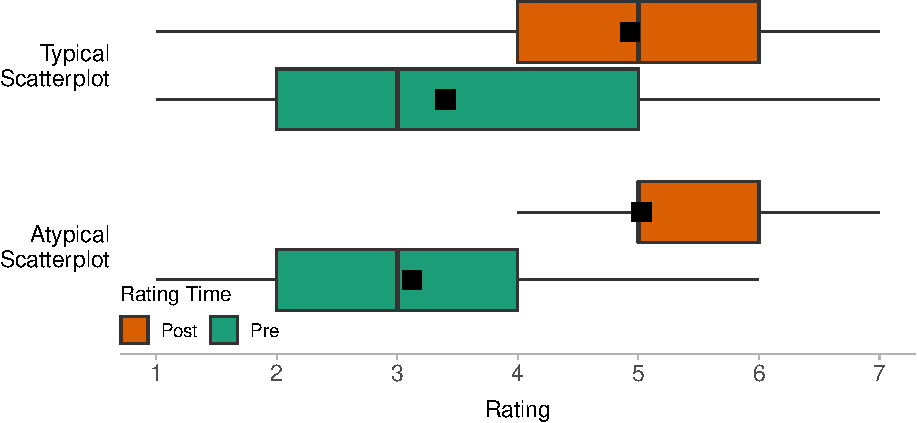
\includegraphics[width=1\textwidth,height=\textheight]{beliefs_attitudes_atypical_scatterplots_files/figure-pdf/fig-abso-descriptives-1.pdf}

}

\caption{\label{fig-abso-descriptives}Boxplots showing ranges,
interquartile ranges, medians (vertical lines) and means for
participants' ratings of strength of relatedness before and after
viewing either typical or atypical scatterplots.}

\end{figure}%

A likelihood ratio test revealed that the model including time of rating
as a predictor explained significantly more variance than the null
(\(\chi^2\)(1) = 8,261.07, \emph{p} \textless{} .001). This model had
random intercepts for participants. Statistical testing providing
support for this hypothesis is shown in Table~\ref{tbl-abso-diff}.
Figure~\ref{fig-abso-descriptives} shows means and boxplots for ratings
of strength of relatedness before and after viewing scatterplots in
either the typical or atypical condition.

Our second hypothesis, that the difference between ratings of strength
of relatedness before and after viewing experimental plots would be
greater when participants were assigned to the atypical scatterplot
condition, also received support. We built a linear mixed effects model
whereby the difference was predicted by the condition the participant
was assigned to. A likelihood ratio test revealed that the model
including condition as a predictor explained significantly more variance
than the null (\(F\)(1) = 72.07, \emph{p} \textless{} .001). This model
contains no random effects terms. Test statistics, along with
semi-partial R\textsuperscript{2} can be seen in Table~\ref{tbl-rel}.

\begin{table}

\caption{\label{tbl-rel}Statistics for the significant main effect of
condition on the difference between pre and post scatterplot viewing
ratings for typical and atypical plots. Semi-partial
R\textsuperscript{2} is also incuded.}

\centering{

\begin{tabular}[t]{lrrrrll}
\toprule
  & Estimate & Standard Error & df & t-value & \textit{p} & R\textsuperscript{2}\\
\midrule
(Intercept) & 1.72 & 0.022 & 2 & 78.22 & <0.001 & \\
Condition & 0.37 & 0.044 & 5998 & 8.49 & <0.001 & 0.012\\
\bottomrule
\end{tabular}

}

\end{table}%

\subsubsection{Additional Analyses}\label{additional-analyses}

\begin{table}

\caption{\label{tbl-lit-stat}Statistics for main effects and
interactions when scores on the Subjective Graph Literacy test are
included in the model.}

\centering{

\begin{tabular}[t]{lrrrrll}
\toprule
  & Estimate & Standard Error & df & t-value & \textit{p} & R\textsuperscript{2}\\
\midrule
(Intercept) & 2.00 & 0.114 & 4 & 17.53 & <0.001 & \\
Condition & -1.36 & 0.228 & 4 & -5.97 & <0.001 & 0.006\\
Literacy & -0.01 & 0.005 & 4 & -2.81 & 0.005 & 0.001\\
Condition * Literacy & 0.08 & 0.010 & 5996 & 7.91 & <0.001 & 0.01\\
\bottomrule
\end{tabular}

}

\end{table}%

\begin{table}

\caption{\label{tbl-dc-stat}Statistics for main effects and interactions
when scores on the Defensive Confidence test are included in the model.}

\centering{

\begin{tabular}[t]{lrrrrll}
\toprule
  & Estimate & Standard Error & df & t-value & \textit{p} & R\textsuperscript{2}\\
\midrule
(Intercept) & 2.15 & 0.146 & 4 & 14.75 & <0.001 & \\
Condition & -1.51 & 0.292 & 4 & -5.17 & <0.001 & 0.004\\
Defensive Confidence & -0.01 & 0.003 & 4 & -3.13 & 0.002 & 0.002\\
Condition * Defensive Confidence & 0.04 & 0.007 & 5996 & 6.57 & <0.001 & 0.007\\
\bottomrule
\end{tabular}

}

\end{table}%

\begin{table}

\caption{\label{tbl-emo-stat}Statistics for main effects and
interactions when likert ratings of topic emotionality are included in
the model.}

\centering{

\begin{tabular}[t]{lrrrrll}
\toprule
  & Estimate & Standard Error & df & t-value & \textit{p} & R\textsuperscript{2}\\
\midrule
(Intercept) & 1.79 & 0.054 & 4 & 33.48 & <0.001 & \\
Condition & 0.68 & 0.107 & 4 & 6.33 & <0.001 & 0.007\\
Topic Emotionality Rating & -0.03 & 0.017 & 4 & -1.58 & 0.115 & 0\\
Condition * Topic Emotionality Rating & -0.11 & 0.034 & 5996 & -3.15 & 0.002 & 0.002\\
\bottomrule
\end{tabular}

}

\end{table}%

We find effects of participants' scores on a Defensive Confidence test
(\(F\)(2) = 23.23, \emph{p} \textless{} .001), participants' scores on a
graph literacy test \citep{garcia_2016} (\(F\)(2) = 39.23, \emph{p}
\textless{} .001), and of how emotional participants' rated the chosen
correlative statement before beginning the block of trials (\(F\)(2) =
5.45, \emph{p} = .004). There are significant fixed and interactive
effects present for both graph literacy and defensive confidence.
Table~\ref{tbl-lit-stat} and Table~\ref{tbl-dc-stat} contain statistics,
including partial R\textsuperscript{2} for both factors respectively. We
found no significant fixed effect of emotionality ratings, but an
interaction was observed, which can be see in Table~\ref{tbl-emo-stat}.
Given the low estimates and effects sizes associated with the fixed
effects of defensive confidence and graph literacy, and the the absence
of a fixed effect of emotionality, we instead choose to focus on the
interactions themselves; see Section~\ref{sec-add-analyses} for further
discussion of these effects.

\subsection{Discussion}\label{discussion}

\subsubsection{Graph Literacy, Defensive Confidence, and Topic
Emotionality}\label{sec-add-analyses}

\begin{figure}

\centering{

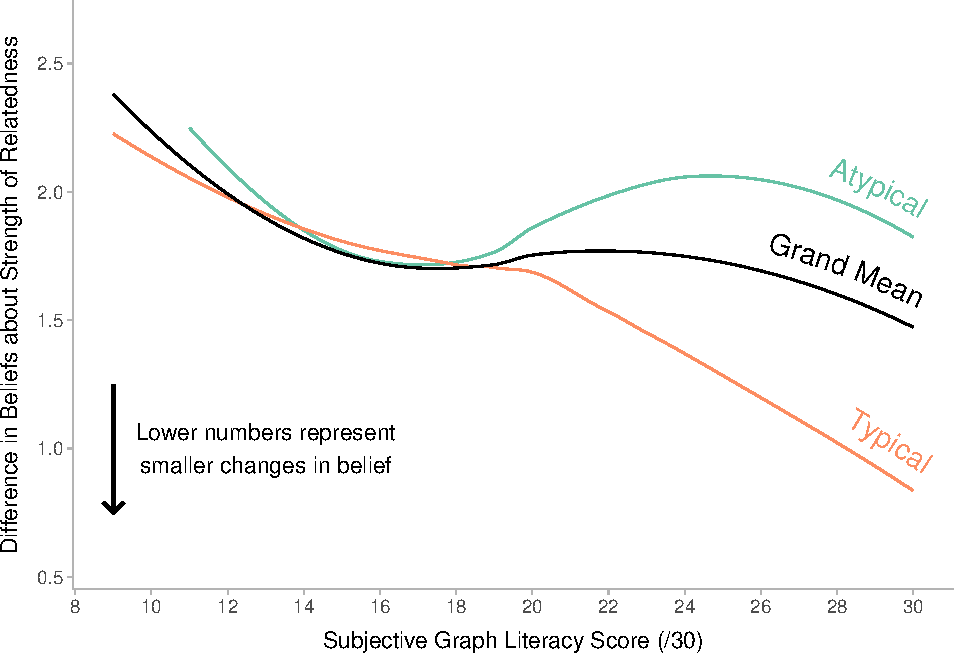
\includegraphics{beliefs_attitudes_atypical_scatterplots_files/figure-pdf/fig-lit-smooth-1.pdf}

}

\caption{\label{fig-lit-smooth}Illustrating how differences in beliefs
about strength of relatedness change as a function of partcipants'
scores on the subjective graph literacy test; smoothed curves are shown
for the grand mean, as well as separately for atypical and typical
scatterplot presentation conditions.}

\end{figure}%

Mean differences in pre and post plot-viewing ratings of strength of
relatedness can be seen in Figure~\ref{fig-lit-smooth}. Generally,
participants who scored higher on a graph literacy test experienced
smaller changes in their ratings of strength of relatedness. While the
effect size associated with this interaction is small
(\textasciitilde0.01, see Table~\ref{tbl-lit-stat}), and does not alter
the overall pattern of results, it is in line with previous work
suggesting that those with higher levels of graph or visualization
literacy show better performance in inference tasks related to
visualizations \citep{canham_2010}, are more capable of describing
effects that visualisations aim to communicate \citep{shah_2011}, and
are able to preferentially attend to relevant features of visualizations
to a greater degree \citep{okan_2015}, than those with lower levels of
graph literacy. In the present study, we provide evidence that those
with greater levels of graph literacy are \emph{less susceptible} to
having their beliefs changed by visualizations, although this difference
is somewhat negated if participants viewed atypical scatterplots, in
which case levels of belief change were relatively consistent. We
hypothesize that this is due to the non-standard nature of the atypical
scatterplots used in that condition.

\begin{figure}

\centering{

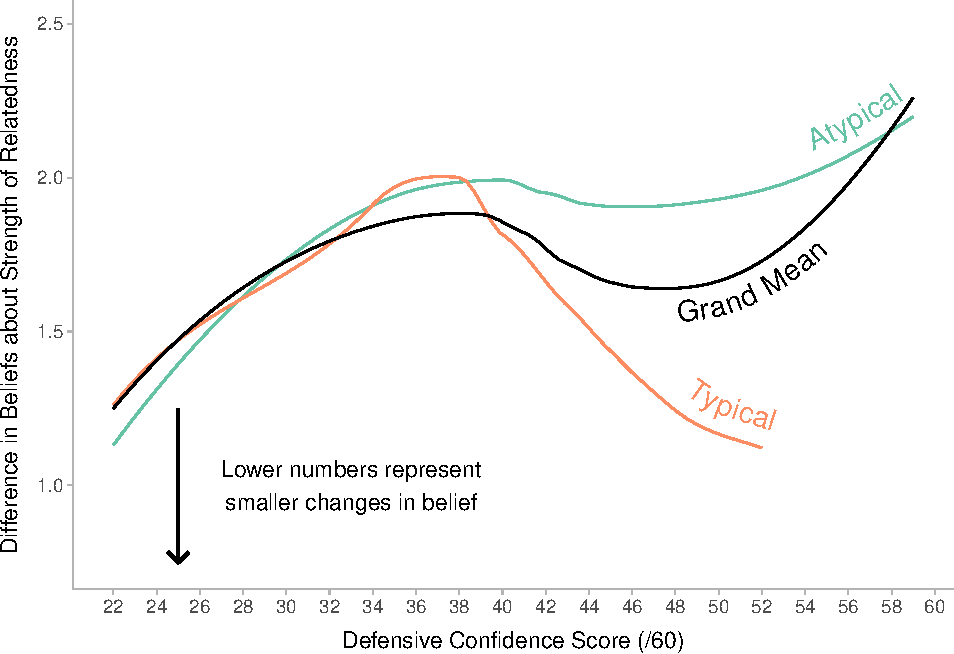
\includegraphics{beliefs_attitudes_atypical_scatterplots_files/figure-pdf/fig-dc-smooth-1.pdf}

}

\caption{\label{fig-dc-smooth}Illustrating how differences in beliefs
about strength of relatedness change as a function of partcipants'
scores on the defensive confidence test; smoothed curves are shown for
the grand mean, as well as separately for atypical and typical
scatterplot presentation conditions.}

\end{figure}%

We observe an opposing pattern of results when examining the effects of
defensive confidence on participants' propensity for belief change.
Generally, participants who scored more highly on the defensive
confidence test experienced greater levels of belief change. This is in
line with evidence that those who are more confidence in their ability
to defend their own beliefs are more liable to having those beliefs
changed in light of evidence \citep{albarracin_2004}. An extended
analysis of the defensive confidence data collected by Markant et al.,
\citep{markant_2023} revealed a similar pattern of results; participants
who scored more highly on a defensive confidence test experienced
greater levels of belief change after viewing scatterplot
visualizations\footnote{The GitHub repository associated with this paper
  contains an R script that performs this analysis.}, although the
effect in that case is much less pronounced due to differences in study
design. This effect is explained as being due to those with a greater
degree of confidence in their own ability to defend their ideas engage
with information with lower levels of attention to the fact it opposes
their beliefs. The present study provides evidence in favour of this
phenomenon.

While the general pattern of results is expected based on previous work,
the interaction present between defensive confidence and scatterplot
condition is novel (see Figure~\ref{fig-dc-smooth}). It would appear
that despite following the normal pattern of results for low to moderate
levels of defensive confidence, those participants who viewed the
typical scatterplots experienced a drop in belief change as defensive
confidence increased past \textasciitilde{} 36/60. There are several
potential explanations in the data; firstly, that the 75 participants
who formed the typical scatterplot presentation group had a more
restricted range of defensive confidence scores, topping out at 52; and
secondly, that the unfamiliar nature of the atypical scatterplots was
protective against against an unexpected, standard behaviour whereby
very high levels of defensive confidence decrease susceptibility to
belief change.

\begin{figure}

\centering{

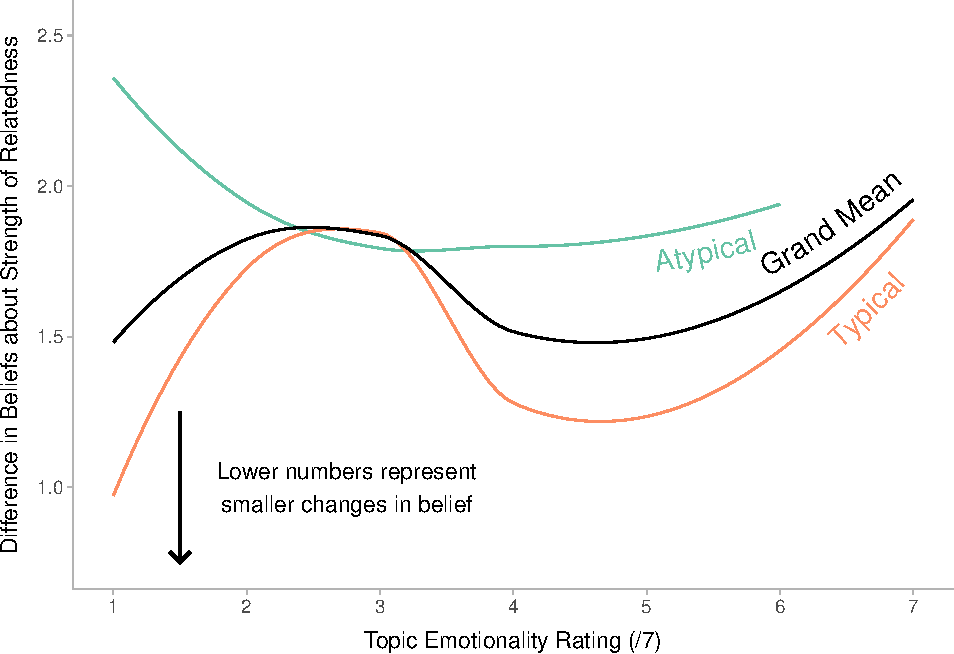
\includegraphics{beliefs_attitudes_atypical_scatterplots_files/figure-pdf/fig-emo-smooth-1.pdf}

}

\caption{\label{fig-emo-smooth}Illustrating how differences in beliefs
about strength of relatedness change as a function of partcipants'
scores on the subjective graph literacy test; smoothed curves are shown
for the grand mean, as well as separately for atypical and typical
scatterplot presentation conditions.}

\end{figure}%

Examining Figure~\ref{fig-emo-smooth}, it would appear that the
interaction we see between belief change and topic emotionality is
driven by those participants who rated the statement low on emotionality
having different levels of belief change between atypical and typical
scatterplot presentation conditions; in this case levels of belief
change were much higher for the group that viewed the atypical
scatterplot designs. There is a broad research space regarding
emotionality and data visualization \citep{lan_2023}, and it is clear
from previous work that emotion affects perception, cognition, and
behaviour \citep[probably look for more]{phelps_2006, harrison_2013}
with regard to data visualization. Harrison et al.~{[}\citet{harrison}
\_2013{]} found that participants who were positively primed performed
better on a low-level visual judgement task. Comparison of this work to
the current is difficult, as \emph{success} on our task is hard to
define. From our data, it is unclear why participants who rated the
correlative statement as ``strongly negative'' experienced significantly
higher levels of belief change when they viewed atypical scatterplots.
We decided to capture the emotionality of the statement simply because
we had done so in the pre-study; we made no predictions based on it, and
chose a broad measure of emotionality, meaning we did not capture
intensity separately from valence. It may be that the strong negative
emotion amplified the effect of scatterplot condition in a way that
strong positive emotion did not, although it is unclear why this has
occurred. Further experimental work is required to provide concrete
explanations for the interactive effects of graph literacy, defensive
confidence, and statement emotionality in the current experimental
paradigm; as the investigation of these is not the prime goal of the
present study, however, we do not consider this a shortcoming.

\section{General Discussion}\label{general-discussion}

\section{Limitations}\label{limitations}

\section{Future Work}\label{future-work}

\begin{itemize}
\tightlist
\item
  maybe something about attitudes
\item
  understanding how DC and literacy interact
\item
  extending beliefs and attitudes to behavioural change (golden ticket
  really)
\end{itemize}

\section{Conclusion}\label{conclusion}

\bibliographystyle{ACM-Reference-Format}
\bibliography{atypical-scatterplots.bib}

%% begin pandoc before-bib
%% end pandoc before-bib
%% begin pandoc biblio
%% end pandoc biblio
%% begin pandoc include-after
%% end pandoc include-after
%% begin pandoc after-body
%% end pandoc after-body

\end{document}
\endinput
%%
%% End of file `sample-manuscript.tex'.
